\acp{vlsd} in general provide high availability and elasticity in a distributed environment composed by a set of commodity hardware. This is a whole new paradigm that avoids the need to invest in very powerful and expensive servers to host the database. In addition, these data stores also provide replication, fail-over, load balancing and data distribution. Also, their data model is more flexible than the relational one since the cost of maintaining its normalized data model, by the enforcement of relations integrity, and the ability to run
transactions across all data in the database make it difficult to scale~\cite{Vilaca:2010:ETL:1926129.1926137}. 

Nevertheless, when compared to \acp{rdbms} which have been widely used over the last 30 years and are therefore much more mature, \ac{vlsd} databases have some fundamental limitations that should be taken into account. They provide high scalability at the expense of a more relaxed data consistency model (usually eventual consistency~\cite{Vogels2008}) and only provide primitive querying and searching capability that do not comply to a standard as is the case of \ac{sql} for \acp{rdbms}. Thus, data abstraction and consistency becomes responsibility of the application developers and the code becomes vendor specific.

In this chapter we will introduce some of the most popular \acp{vlsd} and detail Apache's Cassandra in particular since it was the one we chose to develop our work upon.

\section{Project Voldemort}
Voldemort is an eventually consistent key-value store~\cite{nosqlOrg} written in Java and is an open source implementation of Amazon's Dynamo~\cite{Hastorun2007}. As such, each node is independent of other nodes with no central point of failure or coordination. It is used  at LinkedIn for certain high-scalability storage problems where simple functional partitioning is not sufficient~\cite{voldemort}.

\subsubsection{Data Storage}

Voldemort has a very simple \ac{api} and supports pluggable serialization to allow for rich keys and values to integrate with serialization frameworks like Protocol Buffers, Thrift, Avro, Java Serialization and JSON. 

Also, in order to make the system more resilient to server failure data is replicated through N servers, which means it tolerates up to N-1 failures without losing data. To mitigate the problems that arise with replication, such as multiple updates on different server or a server not being aware of an update do to a crash, Voldemort uses data versioning with vector clocks~\cite{fidge_vector_clocks_1988} that resolve inconsistencies at read time. 

Voldemort's cluster may serve multiple stores and each of them has a unique key space and storage definition, such as serialization method or the storage engine used\footnote{the underlying storage used by Voldemort can be the BerkeleyDB JE, MySQL or read-only stores, others may be used, since it is pluggable}.

\subsubsection{Clustering and Replication}

The request routing in Voldemort is done with consistent hashing\footnote{``Consistent hashing is a scheme that provides hash table functionality in a way that the addition or removal of one slot does not significantly change the mapping of keys to slots. By using consistent hashing, only K/n keys need to be remapped on average, where K is the number of keys, and n is the number of slots.'' in Wikipedia, 13/12/2010}) which assigns nodes to multiple places on the hash ring providing automatic load balance and ability to migrate partitions.

Voldemort provides eventual consistency and as such it focuses on the A (availability) and P (partition tolerance) of the CAP theorem. This trade-off between consistency and availability can be tuned by the client since each of the data stores can have a different number of nodes to which data is replicated, the \textbf{N} value or preference list, and the values \textbf{R} and \textbf{W} for quorum reads and writes, respectively. When reading data, it will read from the first R available replicas in the preference list, return the latest version and repair the obsolete ones. If causality can’t be determined, client side reconciliation is allowed. When writing in quorum, the update is done synchronously for W replicas in the preference list and asynchronously to the others.  

This leads to the inequality \ref{eq:ineq} that provides read-your-writes consistency which is the stronger consistency available.

\begin{equation}
	R + W > N
\label{eq:ineq}	
\end{equation}	

\section{Riak}

Riak is a key-value store~\cite{nosqlOrg} written mostly in Erlang and C, developed by Basho Technologies and is, according to them~\cite{riakWeb}, heavily influenced by the CAP theorem and Amazon's Dynamo paper~\cite{Hastorun2007}. It is master-less, i.e. all nodes in a Riak cluster are equal, each node is fully capable of serving any client request which means that there is no single point of failure. 

\subsubsection{Data Storage}

Riak structures data using buckets, keys and values, being that the values are referenced by a unique key and each key value pair is stored in a bucket. Thus, buckets provide different namespaces making it possible for the keys with the same name to coexist in a Riak cluster.

Its \ac{api} uses \ac{rest} and the storage operations use \ac{http} PUTs and POSTs and fetches use \ac{http} GETs which are submitted to a predefined \ac{url} (default is ``/riak''). In order to take full advantage of this Riak also provides a functionality called links, that are are metadata that establish one-way relationships between objects in Riak and can be used to loosely model graph like relationships between them.

\subsubsection{Clustering and Replication}

Physical servers, referred to in the cluster as \textbf{nodes}, run a certain number of virtual nodes, or \textbf{vnodes}. Each vnode will claim a partition on the ring and the number of active vnodes per node is determined by the number of physical nodes in the a cluster at any given time. 

Each node in the cluster is responsible for 1/(total number of physical nodes) of the ring and the number of vnodes of each node can be determined by calculating (number of partitions)/(number of nodes). As an example consider a ring with 32 partitions, composed of four physical nodes, it will have approximately eight vnodes per node.

Riak's bucket information is communicated across the cluster through a gossip protocol, this includes the \emph{hinted handoff} mechanism used to compensate for failed nodes, in which the failed node neighbors will perform its work, allowing for the cluster to continue to work.  

The number of nodes to which data is replicate, the \textbf{N} value, is defined in a per bucket basis, but all nodes in the same cluster should agree and use the same N value. When reading or writing data, Riak allows the client to supply a value, \textbf{R} and \textbf{W} respectively, that represents the number of nodes which must return results in order for a read or write to be considered successful. 

Since multiple updates can occurs in different nodes, there has to be a way to reconcile an arrive to a mutual consistent state for the system. To do that, this system uses vector clocks to keep track of at what version each object is. More specifically, by looking at two vector clock Riak must determine whether one object is a direct descendant of the other, the objects are direct descendants of a common parent or if the objects are unrelated in recent heritage. With this information it can then proceed to auto-repair data that is out of sync or at least provide the client with an opportunity to reconcile them in an application specific manner. 

Since it first major release Riak adds the support for Secondary Indexes, allowing an application to tag a Riak object with one or more field/value pairs. The object is indexed under these field/value pairs, and the application can later query the index to retrieve a list of matching keys.

\section{Apache HBase}
HBase is a wide column store~\cite{nosqlOrg} modeled after Google's BigTable~\cite{Chang2008} and is written in Java. It is developed as part of Apache Haddop\footnote{\url{http://hadoop.apache.org/}} project providing a fault-tolerant way of storing large quantities of sparse data while providing strong consistency. 

\subsubsection{Data Storage}
HBase stores its data in tables which are composed of rows and columns, being that each column must belong to a specific column family. The row keys are stored in byte-lexicographical order since they are raw byte arrays instead of strings, furthermore within a row the columns are stored in a sorted order.

Each column is versioned and HBase can store multiple version of every cell and does so in decreasing order so that the most recent values are found first, when reading from a store file. This means that when insert or updating a column, the client must specify its name, value and timestamp. 

\subsubsection{Clustering and Replication}
An HBase cluster is composed by a Master node, responsible for telling the clients in which region server to look for the data, multiple region servers, that are responsible for several regions (parts) of the data of the whole cluster. Each region has a log to whom the changes written to before they are actually pushed to disk, this log is then replicated to a distributed file system, Apache's \emph{HDFS}.

This system also depends on running a ZooKeeper cluster that is used to store membership information, which allows to detect dead servers and to perform master election and recovery from failures. For instance the master can be killed and the cluster will continue to function, by finding a new master.

\section{Cassandra}
\label{sec:cassandra}
Cassandra~\cite{will10}, that was created on Facebook, first started as an incubation project at Apache in January of 2009 and is based on Dynamo~\cite{Hastorun2007} and BigTable~\cite{Chang2008}. This system can be defined as an open source, distributed, decentralized, elastically scalable, highly available, fault-tolerant, tuneably consistent, column-oriented database~\cite{hewitt2010cassandra}. 

Cassandra is distributed, which means that it is capable of running on multiple machines while the users see it as if it was running in only one. More than that, Cassandra is built and optimized to run in more than one machine. So much that you cannot take full advantage of all of its features without doing so. In Cassandra, all of the nodes are identical, there is no such thing as a node that is responsible for certain organizing operations, as in BigTable or HBase. Instead, Cassandra features a peer-to-peer protocol and uses gossip to maintain and keep in sync a list of nodes that are alive or dead. 

Being decentralized means that there is no single point of failure, because all the servers are symmetrical. The main advantages of decentralization are that it is easier to use than master/slave and it helps to avoid suspension in service, thus supporting high availability.

Scalability is the ability to have little degradation in performance when facing a greater number of requests. It can be of two types:

\begin{description}
	\item[Vertical] Adding hardware capacity and/or memory
	\item[Horizontal] Adding more machines with all or some of the data so that all of it is replicated at least in two machines. The software must keep all the machines in sync. 
\end{description}

Elastic scalability refers to the capability of a cluster to seamlessly accept new nodes or removing them without any need to change the queries, rebalance data manually or restart the system.

Cassandra is highly available in the sense that if a node fails it can be replaced with no downtime and the data can be replicated through data centers to prevent that same downtime in the case of one of them experiencing a catastrophe, such as an earthquake or flood. 

Consistency essentially means that a read always return the most recently written value, which is guaranteed to happen when the state of a write is consistent among all nodes that have that data (the updates have a global order). Most \acp{vlsd}, including Cassandra, focus on availability and partition tolerance, relaxing the consistency guarantee, providing eventual consistency.  

In the particular case of Cassandra consistency can be considered tuneable in the sense that the number of replicas that will block on an update can be configured on an operation basis by setting the consistency level combined with the replication factor (Section \ref{sec:consistency}).


\subsection{Data Model}
\label{sec:cass_data_model}
Cassandra is a row oriented\footnote{It is frequently referred to as column oriented, but data in Cassandra is actually stored in rows indexed by a unique key, but each row does not need to have the same columns (number or type) as the ones in the same column family.} database system, with a rather complex data model~\cite{sarkissian09}, that is described below.

The basic building block of Cassandra are columns (Fig. \ref{fig:column}) that consist of a tuple with three elements, a name, a value and a timestamp. The name of column can be a string but, unlike its relational counterpart, can also be long integers, UUIDs or any kind of byte array.

\begin{figure}[htb]
  \begin{center}
    \leavevmode
    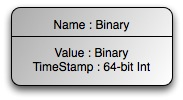
\includegraphics[width=0.3\textwidth]{images/column.jpg}
  \end{center}
  \caption{Cassandra Column}
  \label{fig:column}
\end{figure}

Sets of columns are organized in rows that are referenced by a unique key, the row key, as demonstrated in figure \ref{fig:row}. A row can have any number of columns that are relevant, there is no schema binding it to a predefined structure. Rows have a very important feature, that is that every operation under a single row key is atomic per replica, despite the number of columns affected. This is the only concurrency control mechanism provided by Cassandra.

\begin{figure}[!htb]
  \begin{center}
    \leavevmode
    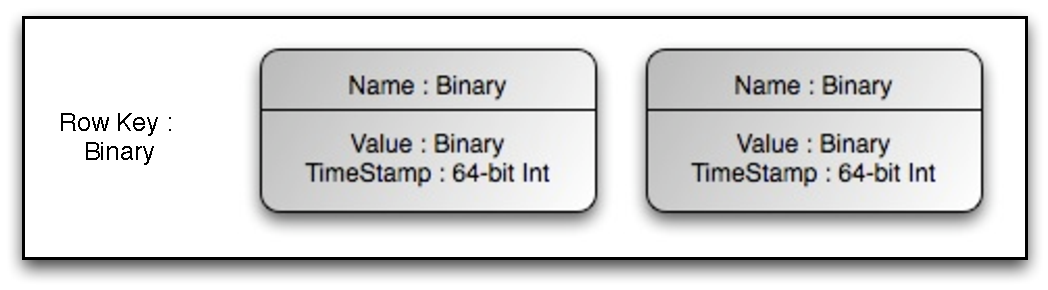
\includegraphics[width=0.8\textwidth]{images/row}
  \end{center}
  \caption{Cassandra Row}
  \label{fig:row}
\end{figure}

The maximum level of complexity is achieved with the column families, which ``glue'' this whole system together, it is a structure that can keep an infinite\footnote{Limited by physical storage space} number of rows, has a name and a map of keys to rows as shown in picture \ref{fig:columnfamily}. 

Applications can specify the sort order of columns within a column family, based on their name, and order them by its value in bytes, converted to an integer or a string, or even as a 16-byte timestamp.

\begin{figure}[!htb]
  \begin{center}
    \leavevmode
    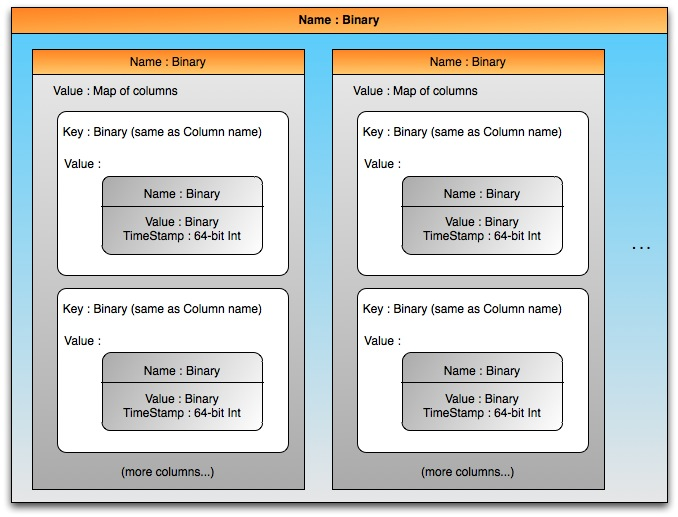
\includegraphics[width=0.8\textwidth]{images/columnfamily}
  \end{center}
  \caption{Cassandra ColumnFamily}
  \label{fig:columnfamily}
\end{figure}


Cassandra also provides another dimension to columns, the SuperColumns (Fig. \ref{fig:supercolumn}), these are also tuples, but only have two elements, the name and the value. The value has the particularity of being a map of keys to columns (the key has to be the same as the column's name).

\begin{figure}[htb]
  \begin{center}
    \leavevmode
    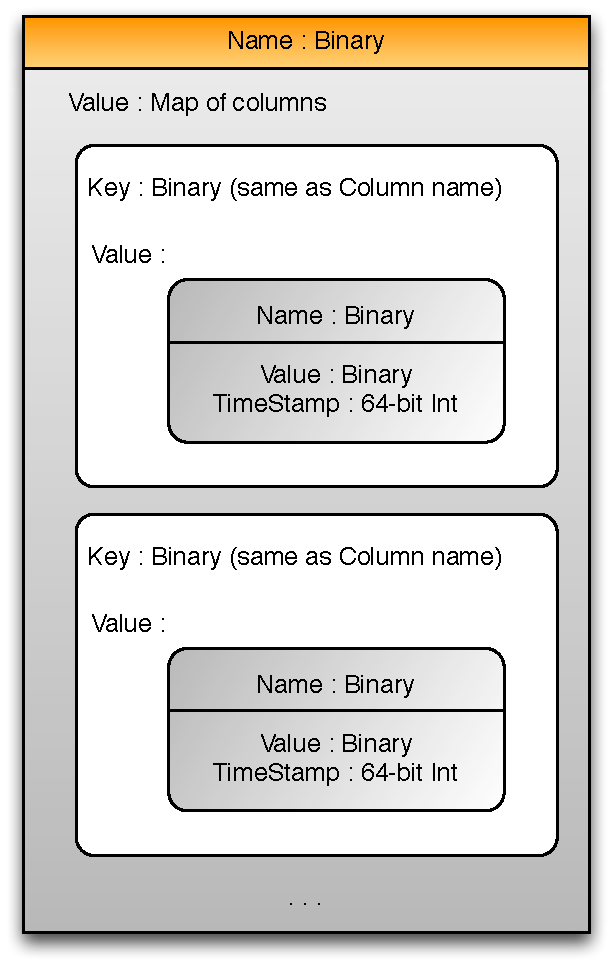
\includegraphics[width=0.4\textwidth]{images/supercolumn}
  \end{center}
  \caption{Cassandra SuperColumn}
  \label{fig:supercolumn}
\end{figure}

There is a variation of ColumnFamilies that are SuperColumnFamilies. The only difference is that where a ColumnFamily has a collection of name/value pairs, a SuperColumnFamily has subcolumns (named groups of columns). This is better understood by looking at the path a query takes until reaching the desired value in both a normal and super column family (Table \ref{tab:path}).

\begin{table}[h!]
\centering
  \begin{tabular}{@{}p{4cm}  r@{}}
	\toprule
	\textbf{Normal} & $Row key \rightarrow Column name \rightarrow Value$\\
    \textbf{Super}  & $Row key \rightarrow Column name \rightarrow Subcolumn name \rightarrow Value$\\
    \bottomrule
  \end{tabular}

\caption{Path to get to value}
\label{tab:path}
\end{table}

Multiple column families can coexist in an outer container called keyspace. The system allows for multiple keyspaces, but most of deployments have only one.

\subsubsection{Partitioners}
\label{sec:partitioners}

Partitioners define the way rows are ordered in Cassandra. By default the one used is the Random partitioner that combines MD5 hashes of the keys with consistent hashing to determine the place where these keys belong in the ring (Section \ref{sec:consistency}). This spreads the keys evenly trough the ring due to its random distribution, but also makes it very inefficient\footnote{most of the times a range query would imply returning the whole set of keys, and filter it.} to perform (even impossible to do from the Cassandra client). 

Since our work relies largely on performing range queries on keys composed of byte arrays, the partitioner used is the Byte-Ordered Partitioner. It is an Order-Perserving Partioner\footnote{Rows are stored by key order, aligning the physical structure of the data with that order} that treats the data as raw bytes, instead of converting it to strings.    


\subsection{Querying}
Cassandra's \ac{api} defines its querying capabilities, and consists of three simple methods\footnote{The actual client API has more methods that are variations of these or schema related}~\cite{lakshmanMalik}:

\begin{itemize}
	\item \emph{insert(table, key, rowMutation)}
	\item \emph{get(table, key, columnName)}
	\item \emph{delete(table, key, columnName)}
\end{itemize}	

In the method signatures above, \emph{columnName} can refer to a specific column in a column family, a column family, normal or super, or a column in a supercolumn. The \emph{rowMutation} specifies the changes to the row in case it was already there, or the row to be added\footnote{Cassandra treats updates as inserts to existent rows, that is the reason there is no update operation}, Mutations can also be Deletions that represent deletes when performing a batch insert.

\subsection{Consistency}
\label{sec:consistency}
Cassandra allows clients to specify the desired consistency level on reads and writes, based on the replication factor previously defined in a configuration file, present in every cluster. Notice that if the inequality \ref{eq:ineq} holds, for R as the number of nodes to block for on read, and W the ones to block for on write, the most consistent behavior will be achieved\footnote{Because the replication process only requires a write to reach a single node to propagate, a write which ``fails'' to meet consistency requirements will still appear eventually as long as it was written to at least one node.}. Obviously his affects the performance and availability, since all update operations must wait for the update to occur in every node.

Cassandra uses replication to achieve high availability and durability. Each data item is replicated at N nodes, where N is the afore mentioned replication factor, assigning each key to a coordinator node (chosen through consistent hashing, that in addition to storing locally each key within his range, replicates these keys at the N-1 nodes in the consistent hashing ring. 

Cassandra system elects a leader amongst its nodes using Zookeeper~\cite{Junqueira2007}, that is contacted by all joining nodes, and tells them for what ranges they are responsible. The leader also makes an effort for maintaining the invariant that no node is responsible for more than N-1 ranges in the ring. 

In Cassandra every node is aware of every other node in the system and, therefore the range they are responsible for.



